% -*- TeX-master: "main"; fill-column: 72 -*-

\newcommand{\fixttspace}{\hspace*{1pt}}

\section{Package syntax and semantics}

In this section, we define the syntax and semantics of the Hierarchical
Model Composition package for SBML Level~3 Version~1.  We expound on the
various data types and constructs defined in this package, then in
\sect{examples}, we provide complete examples of using the constructs in
example SBML models.

\subsection{Namespace URI and other declarations necessary for using this package}
\label{xml-namespace}

Every SBML Level~3 package is identified uniquely by an XML namespace
URI.  For an SBML document to be able to use a given SBML Level~3
package, it must declare the use of that package by referencing its URI.
The following is the namespace URI for this version of the Qualitative Models package for SBML Level~3 Version~1:
\begin{center}
\uri{http://www.sbml.org/sbml/level3/version1/qual/version1}
\end{center}

In addition, SBML documents using a given package must indicate whether
understanding the package is required for complete mathematical
interpretation of a model, or whether the package is optional.  This is
done using the attribute \token{required} on the \token{<sbml>} element
in the SBML document.  For the Qualitative Models package,
the value of this attribute must be set to \val{true}.

The following fragment illustrates the beginning of a typical SBML model
using SBML Level~3 Version~1 and this version of the Qualitative Models package:

\begin{example}
<?xml version="1.0" encoding="UTF-8"?>
<sbml xmlns="http://www.sbml.org/sbml/level3/version1/core" level="3" version="1"
      xmlns:qual="http://www.sbml.org/sbml/level3/version1/qual/version1" qual:required="true">
\end{example}
    

% XML namespace (end)

% -----------------------------------------------------------------------------
\subsection{Primitive data types}
\label{primitive-types}

Section~3.1 of the SBML Level~3 specification defines a number of
primitive data types and also uses a number of XML Schema 1.0 data
types~\citep{biron:2000}.  We assume and use some of them in the rest of
this specification, specifically \primtype{boolean}, \primtype{ID},
\primtype{SId}, \primtype{SIdRef}, \primtype{UnitSId},
\primtype{UnitSIdRef}, and \primtype{string}. The Qualitative Model package defines other primitive types;
they are described below.


\subsubsection{Type \fixttspace\primtypeNC{temporisationType}}
\label{primtype-temporisation}

The \primtype{temporisationType} is an enumeration of values used to indicate the updating policy used by a \Transition.  The possible values are \const{timer}, \const{priority}, \const{sustain}, \const{proportion} and \const{rate}.

\subsubsection{Type \fixttspace\primtypeNC{sign}}
\label{primtype-sign}

The \primtype{sign} is an enumeration of values used to indicate direction of an \Input within the system.  The possible values are \const{positive}, \const{negative} and \const{dual}.

\subsubsection{Type \fixttspace\primtypeNC{transitionInputEffect}}
\label{primtype-inputeffect}
The \primtype{transitionInputEffect} is an enumeration of values used to indicate the effect of an \Input \Transition within the system.  The possible values are \const{none} and \const{consumption}.

\subsubsection{Type \fixttspace\primtypeNC{transitionOutputEffect}}
\label{primtype-outputeffect}
The \primtype{transitionOutputEffect} is an enumeration of values used to indicate the effect of an \Output \Transition within the system.  The possible values are \const{production}, \const{assignmentLevel} and \const{assignmentSymbol}.


% -----------------------------------------------------------------------------
\subsection{The extended \class{Model} class}
\label{model-class}

The extension of SBML Level~3 Core's \Model class is relatively
straightforward: the Qualitative Models Package adds two lists,
one for holding qualitativeSpecies (\qual{listOfQualitativeSpecies}, of class
\ListOfQualitativeSpecies), and the other for holding transitions (\qual{listOfTransitions},
of class \ListOfTransitions).  \fig{} provides the UML
diagram.  The \sbml{Model} element may contain at most one \listOf{QualitativeSpecies}, which must contain at least one \qual{QualitativeSpecies}. It may also contain at most one \listOf{Transitions} which must contain at least one \qual{Transition}.The \QualitativeSpecies class and
the \Transition  class are defined in Sections \sect{qualSpecies-class} and \sect{transitions-class} respectively.

\begin{figure}
  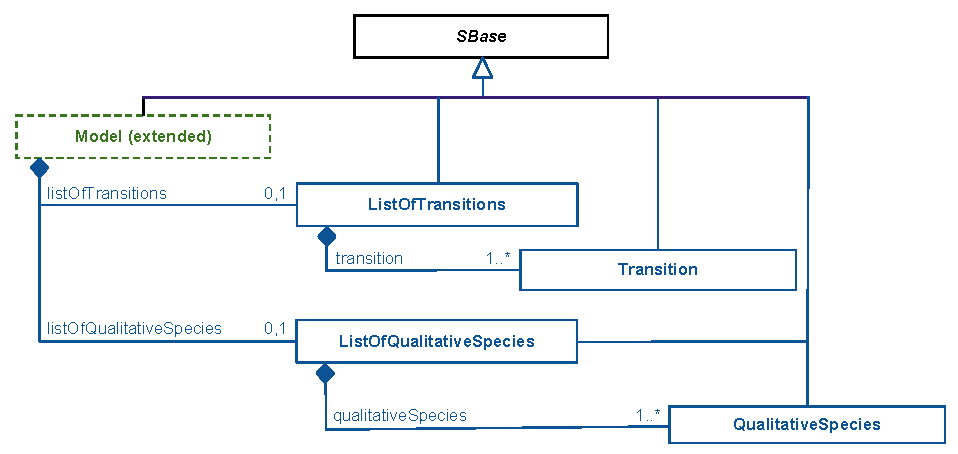
\includegraphics{figs/qual-extended-model-uml.pdf}
  \caption{The definitions of the extended \Model class. In other respects, \Model remains defined as
    in the SBML Level~3 Core specification.}
  \label{qual-extended-model-uml}
\end{figure}


% -----------------------------------------------------------------------------
\subsection{The \class{QualitativeSpecies} class}
\label{qualSpecies-class}
Similarly to the \sbml{Species} in SBML, the components of qualitative models refer to pools of entities that are considered indistinguishable and are each located in a specific \sbml{Compartment}. However, here components are characterised by their qualitative influences rather than by taking parts into reactions. Therefore, we define the \QualitativeSpecies element to represent such pools of entities.

A \QualitativeSpecies describes a pool of indistinguishable entities in a \sbml{Compartment}. It is associated with either a \token{level} or a \token{symbolValue} from its \listOf{SymbolicValues}. \TODO{NEED EXPLANATION OF WHAT THESE STAND FOR} These objects classes are defined in Figure~\ref{qual-qualitative-species-uml}.

\begin{figure}
  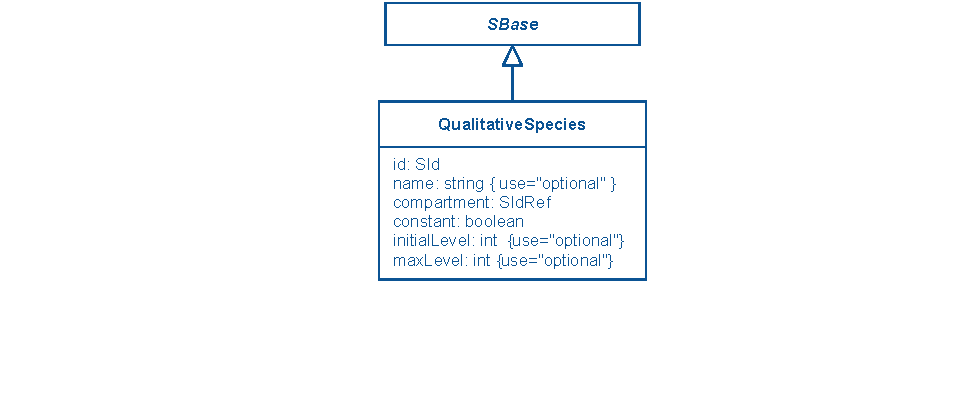
\includegraphics{figs/qual-qualitative-species-uml.pdf}
  \caption{The definitions of the \QualitativeSpecies class. }
  \label{qual-qualitative-species-uml}
\end{figure}


\paragraph{The \fixttspace\token{id} and \fixttspace\token{name} attributes}

The \token{id} attribute takes a required value
of type \primtype{SId}. The \token{id} is used as an identifier for the particluar \QualitativeSpecies.  A \QualitativeSpecies also has an optional \token{name} attribute of type \primtype{string}. 
 The \token{id} and \token{name} attributes may be used
in the same manner as on SBML Level~3 Core
objects; see Section~3.3.2 of the SBML Level~3 Version~1 Core
specification for more information.


\paragraph{The \token{compartment} attribute}
The required attribute \token{compartment}, of type \primtype{SIdRef}, is used to identify the compartment in which the qualitativeSpecies is located.  The attribute's value must be the identifier of an existing \sbml{Compartment} objecyt in the model.  This attribute is comparable with the \token{compartment} attribute on the \sbml{Species} element.

\paragraph{The \token{constant} and \token{boundaryCondition} attributes}
These attributes are treated as in \sbml{Species} elements.

\paragraph{The \token{initialLevel}  attribute:}
The \token{initialLevel} is an \type{integer} that defines the initial level of the \qual{QualitativeSpecies} in its \sbml{Compartment}. This attribute is optional.

\paragraph{The \token{maxLevel} attribute:}
The \token{maxLevel} is an \const{integer} that sets the maximal level of the \qual{QualitativeSpecies}. This attribute is optional.

\subsubsection{The \class{SymbolicValue} class}

% -----------------------------------------------------------------------------
\subsection{The \class{Transition} class}
\label{transitions-class}

\subsubsection{The \class{Input} class}

\subsubsection{The \class{Output} class}

\subsubsection{The \class{FunctionTerm} class}


\subsection{Not yet worked on}

This proposal defines the following new main elements: \qual{QualitativeSpecies}, \qual{SymbolicValue}, \qual{Transition}, \qual{Input}, \qual{Output}, \qual{FunctionTerm}, \qual{DefaultTerm}. All inherit from \sbml{SBase} and all, except \qual{DefaultTerm}, are contained into the corresponding \sbml{ListOf}\textbf{\emph{ElementName}} element, which inherits from \sbml{ListOf}.%, itself inheriting from \sbml{SBase}.

The SBML element \sbml{Model} is extended to include the new elements \listOf{QualitativeSpecies} and \listOf{Transitions}. The SBML elements \sbml{EventAssignment} and \sbml{AssignmentRule} are extended to refer to \qual{QualitativeSpecies}.

The overall structure of this extension is described in Figure~\ref{fig:UML}.

% proposed syntax (end)
\bigskip
\subsection*{Extension of the \sbml{Model} element} % (fold)
\label{sub:model}
The SBML element \sbml{Model} is extended to contain at most one \listOf{QualitativeSpecies} and at most one \listOf{Transitions}.
% subsection model (end)

\subsection*{Definition of \textsf{\textbf{\hypertarget{QualitativeSpecies}{QualitativeSpecies}}}} % (fold)


% subsection qualitativespecies (end)
\bigskip
\subsection*{Definition of \qualt{SymbolicValue}} % (fold)
The \qual{QualitativeSpecies} element may contain at most one \listOf{SymbolicValues} that contains zero or more \qual{SymbolicValue}s. An empty list is allowed, and useful for e.g. adding annotations.
The \qual{SymbolicValue} element defines a non instantiated parameter. Such symbols may represent the different solutions of piecewise linear differential equations, along with different thresholds.

\paragraph{The \token{id} and \token{name} attributes}
These attributes are used according to the SBML L3.1 Section 3.3. The attribute \token{id} is mandatory and \token{name} is optional. 

\paragraph{The \token{rank} attribute}
The \token{rank} is an \type{integer} that defines the position of the symbol in the \listOf{SymbolicValues}. This attribute is optional.

% subsection SymbolicValues (end)
\bigskip
\subsection*{Definition of \qualt{Transition} } % (fold)

A \qual{Transition} element contains at most one \listOf{Inputs}, exactly one \listOf{Outputs} and one \listOf{FunctionTerms}.

\paragraph{The \token{id} and \token{name} attributes:}
These attributes are used according to the SBML L3.1 Section 3.3. They are both optional. 

\paragraph{The \token{temporisationType} attribute:}
The \token{temporisationType} is an \type{enumeration} the "temporisation" of the \qual{Transition}, that is the updating policy associated with the \qual{Transition}. It can be set to \const{timer}, \const{priority}, \const{sustain}, \const{proportion} or \const{rate}.
This attribute is optional. 
% subsection Transitions (end)

\bigskip
\subsection*{Definition of \qualt{Input}} % (fold)
The \listOf{Inputs} contains zero or more \qual{Input}s. A transition with zero inputs can be useful to define an initial assignment, where the state of an output depends on a function but not on any input values. An empty list is allowed, and useful for e.g. adding annotations.
Each \qual{Input} refers to a \qual{QualitativeSpecies} that participates to the corresponding \qual{Transition}.

\paragraph{The \token{id} and \token{name} attributes:}
 These attributes are used according to the SBML L3.1 Section 3.3. They are both optional.

\paragraph{The \token{qualitativeSpecies} attribute:}
The \token{qualitativeSpecies} is a \type{SIdRef} referring to a \qual{QualitativeSpecies}. This attribute is mandatory.

\paragraph{The \token{thresholdLevel} and \token{thresholdSymbol} attributes:}
The \token{thresholdLevel} is an \type{integer} and \token{thresholdSymbol} is a \type{SIdRef}. They are optional and exclusive.

\paragraph{The \token{transitionEffect} attribute:}
The \token{transitionEffect} is an \type{enumeration} describing how the \token{qualitativeSpecies} is affected by the \qual{Transition}. On inputs, the value of \token{transitionEffect} can be either \const{none} or \const{consumption}. (See section \hyperlink{inter_trans}{Interpreting transitions}). This attribute is mandatory.

\paragraph{The \token{sign} attribute}
The \token{sign} is an \type{enumeration} that can be used as an indication on whether the contribution of this input is positive, negative, or both. Thus, possible values can be either \const{positive}, \const{negative} or \const{dual}. The sign is usually used for visualization purposes only. This attribute is optional.

% subsection inputs (end)
\bigskip
\subsection*{Definition of \qualt{Output}} % (fold)
The \listOf{Outputs} contains at least one \qual{Output}.
Each \qual{Output} refers to a \qual{QualitativeSpecies} that participates to the corresponding \qual{Transition}.

\paragraph{The \token{id} and \token{name} attributes:}
These attributes are used according to the SBML L3.1 Section 3.3. They are both optional. 

\paragraph{The \token{qualitativeSpecies} attribute:}
The \token{qualitativeSpecies} is a \type{SIdRef} referring to a \qual{QualitativeSpecies}. This attribute is mandatory.

\paragraph{The \token{outputLevel} attribute:}
The \token{outputLevel} is an \type{integer} used along with the \token{transitionEffect} set to \const{production} to specify the effect of the \qual{Transition} on the corresponding \qual{QualitativeSpecies}. This attribute is optional.

\paragraph{The \token{transitionEffect} attribute:}
The \token{transitionEffect} is an \type{enumeration} describing how the \token{qualitativeSpecies} is affected by the \qual{Transition}. On outputs, the value of \token{transitionEffect} can be \const{production}, \const{assignmentLevel} or \const{assignmentSymbol}. (See section \hyperlink{inter_trans}{Interpreting transitions}). This attribute is mandatory.

% subsection outputs (end)
\bigskip
\subsection*{Definitions of \qualt{FunctionTerm} and \qualt{DefaultTerm}} % (fold)
The \listOf{FunctionTerms} may contain any number of \qual{FunctionTerm} elements, and exactly one \qual{DefaultTerm}. Each term is associated with a result (symbolic or level) and a \qual{FunctionTerm} is associated with a Boolean function inside a \sbml{Math} element. The disjunction of the terms defines the \emph{qualitative function} associated with a \qual{Transition}.

\paragraph{The \token{resultLevel} and \token{resultSymbol} attributes:}
The result of the term is described by a \token{resultLevel} or a \token{resultSymbol}. Both are optional, but one of them must be defined.

The \token{resultLevel} is an \type{integer} describing a level. The \token{resultSymbol} is a \type{SIdRef} referring to a \qual{SymbolicValue}.

\paragraph{The \token{temporisationValue} attribute and the \sbml{TemporisationMath} element:}
The attribute \token{temporisationValue} and the element \sbml{TemporisationMath} allow the specification of the "temporisation" of the \qual{Transition} under the corresponding \qual{FunctionTerm}. Both are optional. Depending on the value of the \token{temporisationType}, either one or both could be used.

The \token{temporisationValue} is a \type{double}. The element \sbml{TemporisationMath} holds a MathML function returning a \type{double}. 

\paragraph{The \sbml{Math} element:}
Each \qual{FunctionTerm} holds a Boolean function encoded in a \sbml{Math} element, using the subset of MathML 2.0 as defined in SBML L3v1 Section 3.4.6.
This element encodes the conditions under which the \qual{FunctionTerm} is selected.


% subsection Terms (end)
\bigskip
\subsection*{\hypertarget{inter_trans}{Interpreting transitions}} % (fold)

\paragraph{Determining the result of a qualitative function:}
The qualitative function associated with a \qual{Transition} is encoded by a \listOf{FunctionTerms}. The \qual{Transition} contains exactly one \qual{DefaultTerm} describing the result of the function by default. A \qual{FunctionTerm} in a \qual{Transition} defines a result (\token{resultLevel} or \token{resultSymbol}) as well as the conditions (\sbml{Math} element) under which this \qual{FunctionTerm} is selected.
The conditions are encoded in MathML as a Boolean function that returns \const{true} if the conditions are fulfilled.
Several \qual{FunctionTerm} elements can have the same result; the qualitative function is then defined as the disjunction of their conditions. 

\paragraph{Encoding the conditions:}
To encode the conditions of the qualitative function, one can use \mathml{ci} elements of MathML to refer to SBML elements. A \mathml{ci} referring to the \token{id} of a \qual{QualitativeSpecies} then refers to the level or the symbol of this \qual{QualitativeSpecies}, while a \mathml{ci} referring to the \token{id} of an \qual{Input} then refers to the \token{thresholdLevel} or the \token{thresholdSymbol} of this \qual{Input}.


\paragraph{The transitionEffect:}
The \qual{Input} and \qual{Output} elements refer to a \qual{QualitativeSpecies} using the attribute \token{qualitativeSpecies}. They are defined with a \token{transitionEffect} attribute that takes one of the following values :
\begin{itemize}
	\item \const{none}: Neither the level nor the symbol associated to the \token{qualitativeSpecies} is modified.
	\item \const{consumption}: The level of the \token{qualitativeSpecies} is decreased by the \token{resultLevel} of the selected term possibly modified by the \token{thresholdLevel} of the \qual{Input}.
	\item \const{production}: The level of the \token{qualitativeSpecies} is increased by the \token{resultLevel} of the selected term possibly modified by the \token{level} of the \qual{Output}.
	\item \const{assignmentLevel}: The level of the \token{qualitativeSpecies} is set to the \token{resultLevel} of the selected term.
	\item \const{assignmentSymbol}: The symbol associated to the \token{qualitativeSpecies} is set to the \token{resultSymbol} of the selected term.
\end{itemize}

% subsection interpreting (end)

